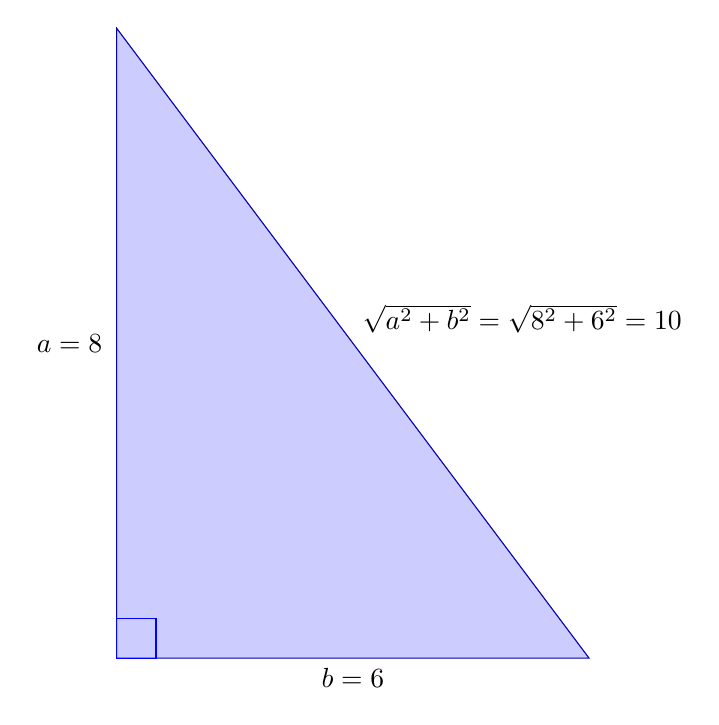
\begin{tikzpicture}

    \filldraw[draw=blue!70!black,fill=blue!20] (0,0) -- (0,8) -- (6,0) -- cycle;
    \draw[blue] (0,0) rectangle (.5,.5);
    \draw (0,4) node [left] {$a=8 \,$};
    \draw (3,0) node [below] {$b=6$};
    \draw (3,4) node [above right] {$\sqrt{a^2 + b^2} = \sqrt{8^2 + 6^2} = 10$};
    
\end{tikzpicture}

% \begin{tikzpicture}[line cap=round,line join=round,>=triangle 45,x=1cm,y=1cm]
% \begin{axis}[
% x=1cm,y=1cm,
% axis lines=middle,
% ymajorgrids=true,
% xmajorgrids=true,
% xmin=-10.68527099647973,
% xmax=23.533276331397282,
% ymin=-10.913759073516744,
% ymax=11.060289507488195,
% xtick={-10,-8,...,22},
% ytick={-10,-8,...,10},]
% \clip(-2,-1) rectangle (2,7);
% \fill[line width=2pt,color=zzttqq,fill=zzttqq,fill opacity=0.10000000149011612] (4.963300016120299,7.402181998049222) -- (-3.7247053187972496,-0.8285598981884658) -- (12.914603144275834,-0.8031563738173618) -- cycle;
% \draw [line width=2pt,color=zzttqq] (4.963300016120299,7.402181998049222)-- (-3.7247053187972496,-0.8285598981884658);
% \draw [line width=2pt,color=zzttqq] (-3.7247053187972496,-0.8285598981884658)-- (12.914603144275834,-0.8031563738173618);
% \draw [line width=2pt,color=zzttqq] (12.914603144275834,-0.8031563738173618)-- (4.963300016120299,7.402181998049222);
% \begin{scriptsize}
% \draw [fill=ududff] (4.963300016120299,7.402181998049222) circle (2.5pt);
% \draw [fill=ududff] (-3.7247053187972496,-0.8285598981884658) circle (2.5pt);
% \draw [fill=ududff] (12.914603144275834,-0.8031563738173618) circle (2.5pt);
% \end{scriptsize}
% \end{axis}
% \end{tikzpicture}